\noindent

\includegraphics[height=1.25cm]{images/pictograms/benchmark}

\includegraphics[height=1.25cm]{images/pictograms/under_construction}

\includegraphics[height=1.25cm]{images/pictograms/FEM}

\includegraphics[height=1.25cm]{images/pictograms/paraview}

%%%%%%%%%%%%%%%%%%%%%%%%%%%%%%%%%%%%%%%%%%%%%%%%%%%%%%%%%%%%%%%%%%%%%%%%%%%%%%%%%%%%%%%%%%%%%%%%%%%

\begin{flushright} {\tiny {\color{gray} python\_codes/fieldstone\_162/text.tex}} \end{flushright}

%\lstinputlisting[language=bash,basicstyle=\small]{python_codes/template_keywords.key}

\par\noindent\rule{\textwidth}{0.4pt}

\begin{center}
\inpython
{\small Code: \url{https://github.com/cedrict/fieldstone/tree/master/python_codes/fieldstone_162}}
\end{center}

\par\noindent\rule{\textwidth}{0.4pt}

{\bf \color{teal} Purpose}: implement and document bla bla 

\par\noindent\rule{\textwidth}{0.4pt}

%%%%%%%%%%%%%%%%%%%%%%%%%%%%%%%%%%%%%%%%%%%%%%%%%%%%%%%%%%%%%%%%%%%%%%%%%%%%%%%%%%%%%%%%%%%%%%%%%%%

According to \textcite{bobf08} (p.90) one can make the ${\bm Q}_1 \times P_0$ stable by adding {\it one}
internal degree of freedom. This then translates as follows:
\begin{eqnarray}
u_h(r,s) &=& 
\overset{\tiny x}{\bN}_1(r,s) u_1 +
\overset{\tiny x}{\bN}_2(r,s) u_2 +
\overset{\tiny x}{\bN}_3(r,s) u_3 +
\overset{\tiny x}{\bN}_4(r,s) u_4 + 
\overset{\tiny x}{\bN}_5(r,s) \alpha \\
v_h(r,s) &=& 
\overset{\small y}{\bN}_1(r,s) v_1 +
\overset{\small y}{\bN}_2(r,s) v_2 +
\overset{\small y}{\bN}_3(r,s) v_3 +
\overset{\small y}{\bN}_4(r,s) v_4 + 
\overset{\small y}{\bN}_5(r,s) \alpha 
\end{eqnarray}
where $\overset{\small x}{\bN_i}$ and $\overset{\small y}{\bN_i}$ 
are the standard $Q_1$ basis functions, $\alpha$ is the additional 
internal dof and 
\begin{eqnarray}
\overset{\small x}{\bN}_5(r,s) &=& r(1-r^2)(1-s^2) \\
\overset{\small y}{\bN}_5(r,s) &=& s(1-r^2)(1-s^2) 
\end{eqnarray}
with
\begin{eqnarray}
\frac{\partial \overset{\small x}{\bN}_5}{\partial r}(r,s) &=& (1-3r^2)(1-s^2) \\
\frac{\partial \overset{\small x}{\bN}_5}{\partial s}(r,s) &=& r(1-r^2)(-2s) \\
\frac{\partial \overset{\small y}{\bN}_5}{\partial r}(r,s) &=& s(-2r)(1-s^2) \\
\frac{\partial \overset{\small y}{\bN}_5}{\partial s}(r,s) &=& (1-r^2)(1-3s^2) 
\end{eqnarray}

Note that in this form the basis functions are not a partition of unity.


%================================
\section*{Implementation}

This is a rather awkward situation where there is only one dof in the center and not two. 
This means that each element has 4x2+1=9 dofs. 
I then logically organise the unknowns/dofs inside an element as follows:
\[
\vec{\cal V}=(u_1,v_1,u_2,v_2,u_3,v_3,u_4,v_4,\alpha)
\]
I then need to carefully go through the derivations of Section~\ref{MMM-sss:KGGT}:
\begin{eqnarray}
\int_\Omega \vec\nabla \vec{\upomega} : {\bm \sigma} \; d\Omega
&=& \int_\Omega \vec\upomega \cdot \vec{b} \; d\Omega 
+ \int_\Gamma \vec\upomega \cdot \vec{t} \; d\Gamma \\
\int_\Omega q \vec\nabla \cdot \vec{\upnu} \; d\Omega &=& 0
\end{eqnarray}
where $\vec\upomega$ and $q$ are the velocity and pressure test functions respectively. 

Since we are going to prescribe the velocity on all sides there is no precribed 
traction on the boundary so that $\int_\Gamma \vec\upomega \cdot \vec{t} \; d\Gamma=0$.

Let us first look at the gradient operator ${\bm B}$:

\begin{eqnarray}
\vec{\dot\varepsilon}_h=
\left(
\begin{array}{c}
\frac{\partial u_h}{\partial r} \\ \\
\frac{\partial v_h}{\partial s} \\ \\
\frac{\partial u_h}{\partial s}\! +\! \frac{\partial v_h}{\partial r} 
\end{array}
\right)
&=&
\left(
\begin{array}{c}
\sum\limits_i  \frac{\partial \overset{\small x}{\bN}_i}{\partial r} u_i + \frac{\partial \overset{\small x}{\bN}_5}{\partial r} \alpha\\ \\
\sum\limits_i  \frac{\partial \overset{\small y}{\bN}_i}{\partial s} v_i + \frac{\partial \overset{\small y}{\bN}_5}{\partial s} \alpha\\ \\
\sum\limits_i (\frac{\partial \overset{\small x}{\bN}_i}{\partial s} u_i + \frac{\partial \overset{\small y}{\bN}_i}{\partial r} v_i) 
+ \frac{\partial \overset{\small x}{\bN}_5}{\partial s} \alpha + \frac{\partial \overset{\small y}{\bN}_5}{\partial r} \alpha
\end{array}
\right) \nn\\
&=&
\underbrace{
\left(
\begin{array}{cccccccccccccccccc}
\frac{\partial \overset{\tiny x}{\bN}_1}{\partial x} & 0 &
\frac{\partial \overset{\tiny x}{\bN}_2}{\partial x} & 0 &
\frac{\partial \overset{\tiny x}{\bN}_3}{\partial x} & 0 &
\frac{\partial \overset{\tiny x}{\bN}_4}{\partial x} & 0 &
\frac{\partial \overset{\tiny x}{\bN}_5}{\partial x} 
\\ \\
0 & \frac{\partial \overset{\tiny y}{\bN}_1}{\partial y} & 
0 & \frac{\partial \overset{\tiny y}{\bN}_2}{\partial y} & 
0 & \frac{\partial \overset{\tiny y}{\bN}_3}{\partial y} & 
0 & \frac{\partial \overset{\tiny y}{\bN}_4}{\partial y} & 
\frac{\partial \overset{\tiny y}{\bN}_5}{\partial y} 
\\ \\ 
\frac{\partial \overset{\tiny x}{\bN}_1}{\partial y} &  
\frac{\partial \overset{\tiny y}{\bN}_1}{\partial x} &  
\frac{\partial \overset{\tiny x}{\bN}_2}{\partial y} &  
\frac{\partial \overset{\tiny y}{\bN}_2}{\partial x} &  
\frac{\partial \overset{\tiny x}{\bN}_3}{\partial y} &  
\frac{\partial \overset{\tiny y}{\bN}_3}{\partial x} &  
\frac{\partial \overset{\tiny x}{\bN}_4}{\partial y} &  
\frac{\partial \overset{\tiny y}{\bN}_4}{\partial x} &  
\frac{\partial \overset{\tiny x}{\bN}_5}{\partial y} + 
\frac{\partial \overset{\tiny y}{\bN}_5}{\partial x} 
\end{array}
\right) 
}_{\bm B}
\!
\cdot
\!
\underbrace{
\left(
\begin{array}{c}
u_1 \\ v_1  \\ u_2 \\ v_2  \\ u_3 \\ v_3 \\ u_3 \\ v_3 \\  \alpha
\end{array}
\right)
}_{\vec{\cal V}} \nn
\end{eqnarray}

I will then focus on the rhs term 
\[
\int_\Omega \vec\upomega \cdot \vec{b} \; d\Omega 
=
\int_\Omega 
(\upomega_x \; \upomega_y) \cdot 
\left(
\begin{array}{c}
b_x \\ b_y
\end{array}
\right)
\; d\Omega 
\]

%We have in the most generic case:
%\begin{eqnarray}
%\upomega_x (x,y)&=& \sum_i \overset{x}{\bN_i}(x,y) \;  \overset{x}{\upomega_i} \\
%\upomega_y (x,y)&=& \sum_i \overset{y}{\bN_i}(x,y) \;  \overset{y}{\upomega_i} 
%\end{eqnarray}
%where $\overset{x}{\bN_i}$ are the basis functions for the $x$-component of the 
%test velocity $\vec{\upomega}$,
%$\overset{y}{\bN_i}$ are the basis functions for the $y$-component of the 
%test velocity $\vec{\upomega}$.
%The sum runs over the dofs inside the element. 

In the case of the ${\bm Q}_1^\star \times P_0$ element we can write the
components of the test function as follows:
\begin{eqnarray}
\upomega_x(x,y) &=& 
\overset{\tiny x}{\bN_1}(x,y) \overset{\tiny x}{\upomega_1}+
\overset{\tiny x}{\bN_2}(x,y) \overset{\tiny x}{\upomega_2}+
\overset{\tiny x}{\bN_3}(x,y) \overset{\tiny x}{\upomega_3}+
\overset{\tiny x}{\bN_4}(x,y) \overset{\tiny x}{\upomega_4}+
\overset{\tiny x}{\bN_5}(x,y) \beta \\
\upomega_y(x,y) &=& 
\overset{\tiny y}{\bN_1}(x,y) \overset{\tiny y}{\upomega_1}+
\overset{\tiny y}{\bN_2}(x,y) \overset{\tiny y}{\upomega_2}+
\overset{\tiny y}{\bN_3}(x,y) \overset{\tiny y}{\upomega_3}+
\overset{\tiny y}{\bN_4}(x,y) \overset{\tiny y}{\upomega_4}+
\overset{\tiny y}{\bN_5}(x,y) \beta 
\end{eqnarray}

\[
\vec{\cal W}^T=
(
\overset{\tiny x}{\upomega_1},\overset{\tiny y}{\upomega_1},
\overset{\tiny x}{\upomega_2},\overset{\tiny y}{\upomega_2},
\overset{\tiny x}{\upomega_3},\overset{\tiny y}{\upomega_3},
\overset{\tiny x}{\upomega_4},\overset{\tiny y}{\upomega_4},\beta)
\]
One can then write
\[
(\upomega_x \; \upomega_y)
=
(
\overset{\tiny x}{\upomega_1},\overset{\tiny y}{\upomega_1},
\overset{\tiny x}{\upomega_2},\overset{\tiny y}{\upomega_2},
\overset{\tiny x}{\upomega_3},\overset{\tiny y}{\upomega_3},
\overset{\tiny x}{\upomega_4},\overset{\tiny y}{\upomega_4},\beta)
\cdot
\left(
\begin{array}{cc}
\overset{x}{\bN_1}(x,y) & 0 \\
0 & \overset{y}{\bN_1}(x,y) \\
\overset{x}{\bN_2}(x,y) & 0 \\
0 & \overset{y}{\bN_2}(x,y) \\
\overset{x}{\bN_3}(x,y) & 0 \\
0 & \overset{y}{\bN_3}(x,y) \\
\overset{x}{\bN_4}(x,y) & 0 \\
0 & \overset{y}{\bN_4}(x,y) \\
\overset{x}{\bN_5}(x,y)  & \overset{y}{\bN_5}(x,y) 
\end{array}
\right)
\]
so that 
\[
(\upomega_x \; \upomega_y) \cdot 
\left(
\begin{array}{c}
b_x \\ b_y
\end{array}
\right)
= 
\vec{\cal W}^T \cdot 
\left(
\begin{array}{cc}
\overset{\tiny x}{\bN_1}(x,y) & 0 \\
0 & \overset{\tiny y}{\bN_1}(x,y) \\
\overset{\tiny x}{\bN_2}(x,y) & 0 \\
0 & \overset{\tiny y}{\bN_2}(x,y) \\
\overset{\tiny x}{\bN_3}(x,y) & 0 \\
0 & \overset{\tiny y}{\bN_3}(x,y) \\
\overset{\tiny x}{\bN_4}(x,y) & 0 \\
0 & \overset{\tiny y}{\bN_4}(x,y) \\
\overset{\tiny x}{\bN_5}(x,y)  & \overset{\tiny y}{\bN_5}(x,y) 
\end{array}
\right)
\cdot
\left(
\begin{array}{c}
b_x \\ b_y
\end{array}
\right)
=
\vec{\cal W}^T \cdot 
\underbrace{
\left(
\begin{array}{c}
b_x\; \overset{\tiny x}{\bN_1}(x,y) \\
b_y\; \overset{\tiny y}{\bN_1}(x,y) \\
b_x\; \overset{\tiny x}{\bN_2}(x,y) \\
b_y\; \overset{\tiny y}{\bN_2}(x,y) \\
b_x\; \overset{\tiny x}{\bN_3}(x,y) \\
b_y\; \overset{\tiny y}{\bN_3}(x,y) \\
b_x\; \overset{\tiny x}{\bN_4}(x,y) \\
b_y\; \overset{\tiny y}{\bN_4}(x,y) \\
b_x\; \overset{\tiny x}{\bN_5}(x,y) +b_y\; \overset{\tiny y}{\bN_5}(x,y) 
\end{array}
\right)
}_{\vec{f}}
\]

Finally let us turn to the $\G$ block.
We have in the general case:
\[
q = \vec{\bN}_p^T \cdot \vec{\cal Q}
\]
where $\vec{\bN}_p$ is the vector\footnote{Remember that by 
default all vectors are column vectors.} (of size $(m_P,1)$) 
of pressure basis functions
and $\vec{\cal Q}$ is the vector (of size $(m_P,1)$) of test pressure dofs.

Let us now turn to the mass conservation equation.
Since $\vec{\bN}_p^T \cdot \vec{\cal Q}= \vec{\cal Q}^T \cdot \vec{\bN}_p$ then
\[
\int_\Omega q \vec\nabla \cdot \vec{\upnu} \; d\Omega 
=\int_\Omega \vec{\cal Q}^T \cdot \vec{\cal N}^p \vec\nabla \cdot \vec{\upnu} \; d\Omega  
=\vec{\cal Q}^T \cdot \int_\Omega \vec{\cal N}^p \vec\nabla \cdot \vec{\upnu} \; d\Omega  
\]
We have 
\begin{eqnarray}
\vec\nabla \cdot \vec{\upnu} 
&=&
\dot \varepsilon_{xx}(\vec\upnu) + \dot \varepsilon_{yy}(\vec\upnu) \\
&=& 
\left(
\begin{array}{ccc}
1 & 1  & 0 
\end{array}
\right)
\cdot
\left(
\begin{array}{c}
\dot \varepsilon_{xx}(\vec\upnu) \\
\dot \varepsilon_{yy}(\vec\upnu) \\
2\dot \varepsilon_{xy}(\vec\upnu)
\end{array}
\right) \nonumber\\
&=&
\left(
\begin{array}{ccc}
1 & 1 & 0 
\end{array}
\right)
\cdot
\vec{\dot \varepsilon}(\vec\upnu)  \nonumber\\
&=&
\left(
\begin{array}{ccc}
1 & 1 & 0 
\end{array}
\right)
\cdot
{\bm B} \cdot \vec{\cal V}
\end{eqnarray}
so that
\begin{eqnarray}
\vec{\cal N}^p  \vec\nabla \cdot \vec{\upnu}
&=& \vec{\cal N}^p  
\left(
\begin{array}{ccc}
1 & 1 & 0 
\end{array}
\right)
\cdot
{\bm B} \cdot \vec{\cal V} \nonumber\\
&=&
\underbrace{
\left(
\begin{array}{cccccc}
\vec{\cal N}^p & \vec{\cal N}^p & 0 
\end{array}
\right)
}_{{\bm \bN}^T}
\cdot
{\bm B} \cdot \vec{\cal V} \nonumber\\
&=&
{\bm \bN}^T \cdot {\bm B} \cdot \vec{\cal V}
\end{eqnarray}
where ${\bm N}_p$ is a $(m_p \times 3)$ matrix.
Finally
\begin{eqnarray}
\int_\Omega q \vec\nabla \cdot \vec{\upnu} \; d\Omega 
&=& \vec{\cal Q}^T \cdot \int_\Omega {\bm \bN}^T \cdot {\bm B} \; d\Omega \cdot \vec{\cal V} \nonumber\\
&=& - \vec{\cal Q}^T \cdot \mathbb{G}^T \cdot \vec{\cal V} 
\end{eqnarray}
where
\[
\mathbb{G} = -\int_\Omega {\bm B}^T \cdot {\bm \bN}\; d\Omega 
\]
In the case of the ${\bm Q}_1^\star \times P_0$ element there is only one pressure dof per element 
so that the corresponding pressure basis function is simply constant and equal to 1. 
Then 
\[
{\bm \bN} = 
\left(
\begin{array}{c}
1 \\ 1 \\ 0
\end{array}
\right)
\]
and 
\[
{\bm B}^T \cdot {\bm \bN} 
=
\left(
\begin{array}{cccccccccccccccccc}
\frac{\partial \overset{x}{\bN}_1}{\partial x} & 0 &
\frac{\partial \overset{x}{\bN}_2}{\partial x} & 0 &
\frac{\partial \overset{x}{\bN}_3}{\partial x} & 0 &
\frac{\partial \overset{x}{\bN}_4}{\partial x} & 0 &
\frac{\partial \overset{x}{\bN}_5}{\partial x} 
\\ \\
0 & \frac{\partial \overset{\tiny y}{\bN}_1}{\partial y} & 
0 & \frac{\partial \overset{\tiny y}{\bN}_2}{\partial y} & 
0 & \frac{\partial \overset{\tiny y}{\bN}_3}{\partial y} & 
0 & \frac{\partial \overset{\tiny y}{\bN}_4}{\partial y} & 
\frac{\partial \overset{\tiny y}{\bN}_5}{\partial y} 
\\ \\ 
\frac{\partial \overset{\tiny x}{\bN}_1}{\partial y} &  
\frac{\partial \overset{\tiny y}{\bN}_1}{\partial x} &  
\frac{\partial \overset{\tiny x}{\bN}_2}{\partial y} &  
\frac{\partial \overset{\tiny y}{\bN}_2}{\partial x} &  
\frac{\partial \overset{\tiny x}{\bN}_3}{\partial y} &  
\frac{\partial \overset{\tiny y}{\bN}_3}{\partial x} &  
\frac{\partial \overset{\tiny x}{\bN}_4}{\partial y} &  
\frac{\partial \overset{\tiny y}{\bN}_4}{\partial x} &  
\frac{\partial \overset{\tiny x}{\bN}_5}{\partial y} + 
\frac{\partial \overset{\tiny y}{\bN}_5}{\partial x} 
\end{array}
\right)^T 
\cdot \left(
\begin{array}{c}
1 \\ 1 \\ 0
\end{array}
\right)
=
\left(
\begin{array}{c}
\frac{\partial \overset{x}{\bN}_1}{\partial x} \\ \\
\frac{\partial \overset{y}{\bN}_1}{\partial y} \\ \\
\frac{\partial \overset{x}{\bN}_2}{\partial x} \\ \\
\frac{\partial \overset{y}{\bN}_2}{\partial y} \\ \\
\frac{\partial \overset{x}{\bN}_3}{\partial x} \\ \\
\frac{\partial \overset{y}{\bN}_3}{\partial y} \\ \\
\frac{\partial \overset{x}{\bN}_4}{\partial x} \\ \\
\frac{\partial \overset{y}{\bN}_4}{\partial y} \\ \\
\frac{\partial \overset{x}{\bN}_5}{\partial x} + 
\frac{\partial \overset{y}{\bN}_5}{\partial y} 
\end{array}
\right)
\]



There are in total $NfemV=NV*ndfoV+nel$ velocity degrees of freedom and $NfemP=nel$
pressure degrees of freedom.


Imposing boundary conditions is rather 
straightforward since the additional dofs are never on the boundary. 

When it comes to quadrature, the velocity basis functions contain quadratic 
terms so we'll use a $3\times 3$ quadrature for the $\K$ block. 
However it is made clear by the authors that the bilinear form responsible for $\G$ 
must be underintegrated (1 point quadrature). 


The code for this stone is based on \stone~14.


Remark: Since the additional dofs are internal one could resort to static condensation
so as to reduce the size of the FEM system $\K$ block.

\begin{center}
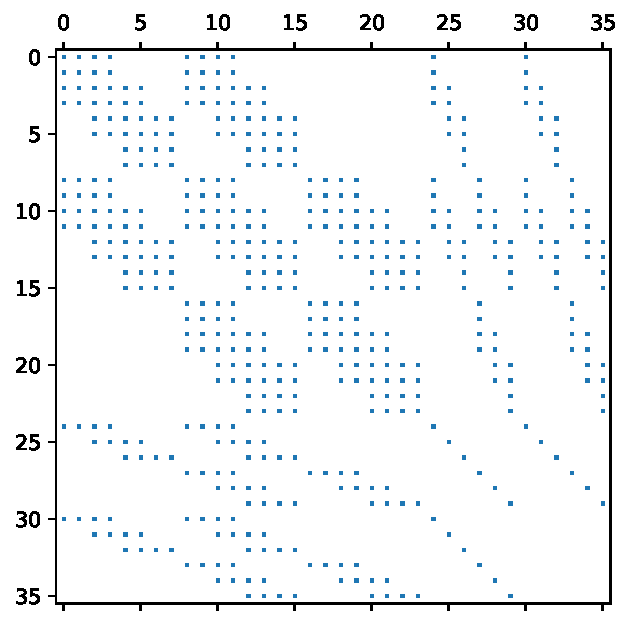
\includegraphics[width=6cm]{python_codes/fieldstone_162/images/matrix.pdf}\\
{\captionfont nonzero pattern for a $3\times 2$ mesh.}
\end{center}

%============================================
\section*{Results}





